\chapter{Representación y visualización de superficies implícitas}

Tras el primer capítulo donde introdujimos el concepto de superficie implícita y distintos métodos para, a partir de superficies expresadas en forma paramétrica, obtener la expresión implícita de ésta. Nos cabe preguntarnos cuáles son los métodos más básicos para poder representar las superficies en forma implícita.

Claro está que estos métodos no tienen por qué ser los mejores computacionalmente hablando, pero nos dan una primera aproximación al tema principal de este Trabajo Fin de Máster.

Por tanto en este capítulo se basará en presentarnos dos métodos de visualización: poligonalización, para lo cual explicaremos un algoritmo en detalle, y Ray Tracing.

\section{Representación de superficies algebraicas y blobs}

\subsection{Superficies algebraicas}

Una superficie se dice algebraica si se define por polinomios cuyo grado refleja el grado de la superficie. El grado indica el número de intersecciones de la superficie y una recta, véase \cite{Bloomenthal97}. Por ejemplo un plano tiene grado 1 mientras que una esfera tiene grado 2. El uso de polinomios tiene la ventaja de ser menos costoso, en tiempo de renderización, que cualquier otra representación analítica general.

Las superficies algebraicas más utilizadas son las cuadráticas. Este tipo de superficies son fáciles de renderizar, son necesarios muy pocos parámetros para controlar su forma y, además, es posible usar coordenadas homogéneas para aplicar transformaciones afines. A continuación mostramos típicas superficies cuadráticas como son la esfera, el cilindro y el cono.
\begin{figure}[h]
	\centering
	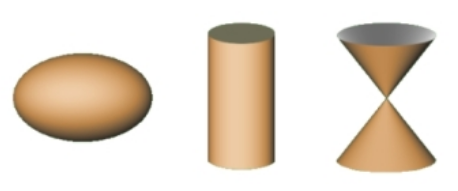
\includegraphics[scale=0.7]{images/florez4.png}
	\caption{Ejemplos básicos de superficies cuadráticas.}
\end{figure}

\subsection{Blobs}

Los blobs son sumas de distribuciones gaussianas inspiradas en la distribución de densidad de las moléculas. Este tipo de superficies fueron usadas por primera vez por Blinn \cite{Blinn82} para renderizar una animación del ADN para el programa de televisión Cosmos de Carl Sagan, en donde cada átomo era aproximado por una esfera gaussiana.

La suma de esferas gaussianas genera una unión entre las superficies. Blinn propuso la función
\begin{equation}
f(x,y,z) = \sum_{i=1}^{n} b_i e^{-a_i r_i(x,y,z)^2} - T,
\nonumber
\end{equation}
donde cada sumando está centrado en un término $r_i$ y $T$ representa el umbral. El término $r_i$ se calcula como
$$r_i(x,y,z) = \sqrt{(x - x_i)^2 + (y-y_i)^2 + (z-z_i)^2}.$$
El término $b$ representa la altura de la función y el término $a$ es la desviación estándar. El efecto de la función blob se puede modificar cambiando los parámetros.
\begin{figure}[h]
	\centering
	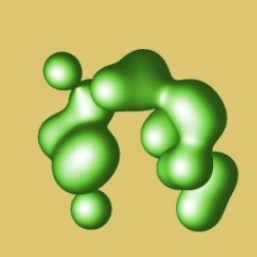
\includegraphics[scale=0.7]{images/florez3.png}
	\caption{Ejemplo de sumas de esferas gaussianas.}
\end{figure}

La función exponencial define una esfera gaussiana que tiende a infinito a la par que la exponencial tiende a cero. Esto significa que cada esfera gaussiana influye sobre las demás sin importar la separación que exista entre ellas. Los objetos flexibles\cite{Wyvill86} computan las esferas usando aproximaciones polinomiales.
\newpage
\section{Métodos de visualización}

En esta sección cubrimos dos de los métodos de visualización usados y referenciados en la bibliografía de superficies implícitas de forma más frecuente: poligonalización y Ray Tracing. Cubriremos ambos con detalle, pero cabe destacar que en el resto del Trabajo Fin de Máster nos centraremos en el desarrollo del segundo.

\subsection{Poligonalización de superficies implícitas}

La idea general de los métodos de poligonalización consiste en la creación de polígonos que representen la superficie implícita. Los polígonos son fáciles de renderizar en los sistemas gráficos modernos, por tanto, este método suele ser el elegido cuando vamos a realizar visualización interactiva.

Existen varios métodos  de poligonalización de superficies, siendo los más populares:
\begin{itemize}
\item El llamado{ \em método de las celdas fijas}\cite{Bloomenthal90} consistente en dividir el espacio en poliedros de forma conveniente (cubos, tetraedros,...) y, tras esto, en calcular la intersección de la superficie con  las aristas de los poliedros para así definir los vértices de la poligonalización. Estos vértices han de ordenarse para crear polígonos convexos.

Obviamente la calidad del resultado depende en gran medida de como de { \em fina} sea la división del espacio, esto es, si los poliedros son demasiado grandes entonces se perderán una gran cantidad de detalles y si son demasiado pequeños crearán polígono en exceso que realentizarán la renderización.

Este problema se puede solucionar con una serie de métodos adaptativos donde el tamaño de la celda según el detalle de la superficie, véase, si en una zona nos interesa hacer una poligonalización más detallada allí habrá una división más fina. Aunque estos métodos son difíciles de implementar y aún no son muy populares por esta razón y las celdas de tamaño fijo suelen ser la opción más común.

\item El segundo método más común son los{ \em marching methods} que consisten en crear, de forma sucesiva, un mallado triangular comenzando con un punto o un polígono dado. Este método lo explicaremos mejor a continuación con un ejemplo claro donde mostraremos un algoritmo concreto extraído de \cite{Hartmann03}.
\end{itemize}

\subsection{El algoritmo de triangulación}

La formulación del algoritmo de triangulación extraído de \cite{Hartmann03}\footnote{Al aparecer en \cite{Hartmann98} los derechos pertenecen a Springer-Verlag.} no usa ninguna representación especial de la superficie para ser triangulada. Las operaciones dependientes de la representación están implícitamente en el apartado de \texttt{surfacepoint} que se define a continuación. En él presentaremos las ideas básicas del algoritmo. Después introduciremos el procedimiento \texttt{surfacepoint} y la estructura de los datos usados. Finalmente se explicaremos los pasos del algoritmo en detalle.


\subsubsection{La idea del algoritmo}

\begin{enumerate}
\item[S0] Escoge un punto $s$ cercano a la superficie. Determina el correspondiente punto $p_1$ de la superficie. Rodea $p_1$ de un hexágono regular $q_2, \dotso, q_7$ en el plano tangente. Con el procedimiento \texttt{surfacepoint} determina los puntos $p_2, \dotso, p_7$ correspondientes a los  puntos iniciales $q_2, \dotso, q_7$.
Ya hemos construido los primeros seis triángulos de la triangulación.
Entonces al conjunto ordenado de puntos $p_2, \dotso, p_7$ lo llamaremos{ \em polígono delantero actual} $\Pi_0$. Si la triangulación se puede limitar por curvas cerradas $\Gamma_1, \Gamma_2,\dotso$ podemos determinar los polígonos delanteros $\Pi_1, \Pi_2, \dotso$ ligados a las curvas.
\begin{figure}[h]
	\centering
	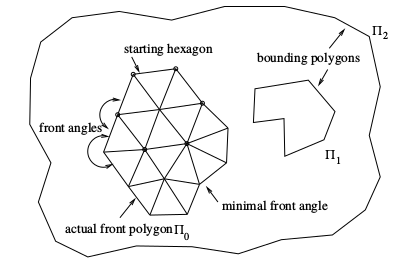
\includegraphics[scale=0.7]{images/hartmann1.png}
	\caption{Nociones básicas del algoritmo de triangulación.}
\end{figure}	
	
\item[S1] Para cada punto del polígono $\Pi_0$ determinamos el ángulo del área aún por triangular. A estos ángulos los llamamos{ \em ángulos delanteros}.
	
\item[S2] Revisamos si algún punto $p_i$ de $\Pi_0$ está cerca. Con cerca entendemos:
\begin{itemize}
	\item Un punto de $\Pi_0$  distinto de $p_i$ y de su entorno.
	\item Un punto de cualquier otro polígono $\Pi_k$ distinto.
\end{itemize}
En el primer caso dividimos el polígono $\Pi_0$ en dos nuevos polígonos $\Pi_0$ y $\Pi_1$. En el segundo caso unimos los dos polígonos en uno nuevo al que llamaremos $\Pi_0$ y será nuestro nuevo polígono delantero actual.

\item[S3] Determinar un punto $p_m$ del polinomio $\Pi_0$ con un ángulo delantero mínimo. Rodea $p_m$ por triángulos con ángulos cercanos a $\frac{\pi}{6}$. Elimina $p_m$ del polígono $\Pi_0$ e inserta los nuevos puntos en $\Pi_0$.

\item[S4] Repite los pasos 1, 2 y 3 hasta que $\Pi_0$ consista sólo en tres puntos que generan un nuevo triángulo. Si aún queda algún polígono restante se convierte en el nuevo $\Pi_0$ y se repiten los pasos 1, 2 y 3. Una vez ya no queden más polígonos, habremos terminado y la triangulación estará completada.
\end{enumerate}

\begin{figure}[h]
	\centering
	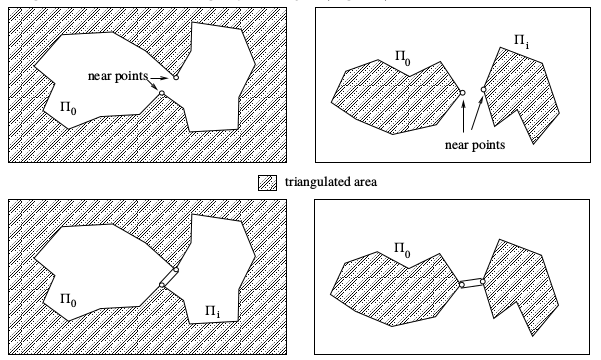
\includegraphics[scale=0.5]{images/hartmann2.png}
	\caption{Dividiendo y uniendo el polígono $\Pi_0$.}
\end{figure}

\subsubsection{El procedimiento \texttt{surfacepoint}}

Un paso fundamental del algoritmo es determinar el punto $p$ de la superficie que está cerca de un punto $q$ en un entorno de la superficie. El vector $q - p$ no ha de ser necesariamente perpenticular a la superficie. Debido a que casi todas las superficies pueden ser numéricamente implicitadas, daremos a solución para superficies implícitas.

Comenzamos con una superficie implícita $\Phi$ definida por una función $f(x) = 0$ para la cual su gradiente $\nabla f$ existe y no se anula para ningún punto de la superficie y un punto $q$ en un entorno de la superficie.
El siguiente procedimiento calcula un punto de la superficie $p$, un normal y dos vectores tangentes al punto $p$.

\begin{enumerate}
	\item
\begin{itemize}
	\item $u_0 := q$.
	\item Repetir $u_{k+1} := u_k - \frac{f(u_k)}{\nabla f(u_k)^2} \nabla f(u_k)$ hasta que $\| u_{k+1} - u_k \|$ es suficientemente pequeño.
	\item $p := u_{k+1}$.
\end{itemize}
	
	\item Definimos el normal a la superficie en $p$ como $n := \frac{\nabla f(p)}{\| \nabla f(p) \|}$.
	
	\item Para los vectores tangentes:
\begin{itemize}
	\item $t_1 := \frac{1}{\| \sqrt{n_x^2 + n_y^2} \|} (n_y, -n_x, 0)$ si $n_x > 0.5$ ó $n_y > 0.5$.
	\item En otro caso elegimos $t_1 := \frac{1}{\| \sqrt{n_x^2 + n_z^2} \|} (-n_z, 0, n_x)$.
	\item $t_2 := n \times t_1$.
\end{itemize}
\end{enumerate}

\subsubsection{La estructura}

Para la construcción de los triángulos necesitamos un paso de longitud $\delta_t > 0$ que es aproximadamente la longitud de las aristas.

Para cada punto $p_i$ guardamos la siguiente información:
\begin{itemize}
	\item Las coordenadas.
	\item El normal y los tangentes a la superficie en $p_i$ tales que son ortonormales entre sí.
	\item El ángulo delantero de $p_i$ si es un punto delantero de $\Pi_0$.
	\item La variable booleana \texttt{angle\_changed} con \texttt{angle\_changed = true} si el ángulo delantero cambió y tiene que ser recalculado.
	\item La variable booleana \texttt{border\_point}, con el valor \texttt{true} si el punto $p_i$ es en el borde de la triangulación y debería ser ignorado para futuros cálculos.
\end{itemize}
Los triángulos serán numerados de forma consecutiva. Para cada triángulo guardaremos el valor numérico de sus vértices.

\subsubsection{S0}

Sea $s$ un punto inicial en un entorno de la superficie. Entonces \texttt{surfacepoint} nos determina el primer punto $p_1$ de la triangulación y el sistema ortonormal $n_1, t_{11} \text{ y } t_{12}$. El resto de puntos $p_2, \dotso, p_7$ son el resultado de aplicar \texttt{surfacepoint} a
$$q_{i+2} = p_1 + \delta_t cos\left(\frac{i \pi}{3}\right)t_{11} + \delta_t sen\left(\frac{i\pi}{3}\right)t_{12}, \hspace{1cm} i = 0, \dotso, 5.$$

Ya hemos obtenido los primeros seis triángulos.

\subsubsection{S1}

Si un punto $p_{0i}$ del polígono delantero $\Pi_0 = (p_{01}, \dotso, p_{0N_0})$ acaba de ser incluido o un punto cercano a $p_{0i}$ es un nuevo punto, entonces es necesario recalcular el ángulo delantero $\omega$ del punto $p_{0i}$. Sea:
\begin{itemize}
	\item $v_1 := p_{0,i-1}$ si $i>1$ ó $v_1 := p_{0N_0}$ si $i=1$.
	\item $v_2 := p_{0,i+1}$ si $i<N_0$ ó $v_2 := p_{01}$ si $i=N_0$.
	\item $(\xi_1,\eta_1,\zeta_1)$ y$(\xi_2,\eta_2,\zeta_2)$ las coordenadas de $v_1$ y $v_2$, respectivamente, en el sistema local ortonormal $n, t_1$ y $t_2$ en el punto $p_{0i}$.
	\item $\omega_i$ el ángulo polar de $(\xi_i, \eta_i)$. 
\end{itemize}
Entonces el ángulo delantero en el punto $p_{0i}$ es $\omega = \omega_2 - \omega_1$ si $\omega_2 \geq \omega_1$ ó $\omega = \omega_2 - \omega_1 + 2\pi$ en caso contrario.

\subsubsection{S2}

Para prevenir el solapamiento de nuevos triángulos sobre los ya existentes comprobaremos:
\begin{itemize}
\item Las distancias dos a dos de los puntos que componen $\Pi_0$. Si hay puntos $p_{0i}$ y $p_{0j}$, con $i<j$, que no son vecinos, ni vecinos de vecino y $\| p_{0i} - p_{0j} \| < \delta_t$ entonces $\Pi_0$ se separa en dos polígonos.
\item Las distancias de puntos de $\Pi_0$ a puntos del resto de polígonos $\Pi_k$. Si hay puntos $p_{0i} \in \Pi_0$ y $p_{mj} \in \Pi_m$ tales que $\| p_{0i} - p_{mj} \| < \delta_t$, entonces los polígonos $\Pi_0$ y $\Pi_m$ se unen.
\end{itemize}
\begin{figure}[h]
\centering
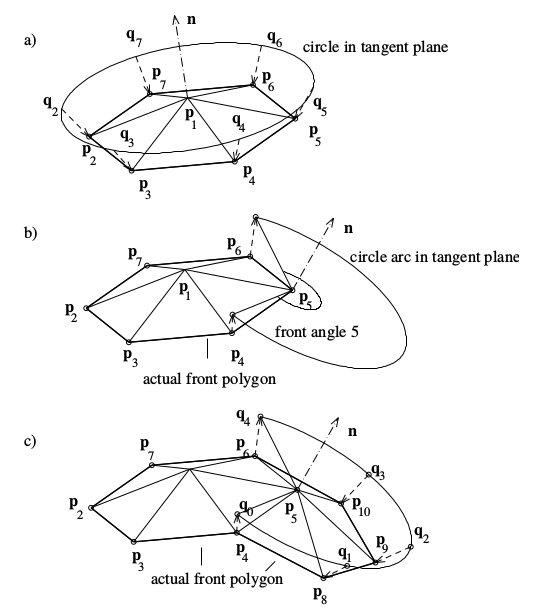
\includegraphics[scale=0.5]{images/hartmann3.png}
\caption{Los primeros pasos del algoritmo.}
\end{figure}

\newpage
\subsubsection{S3}

Sea $p_{0m}$ un punto de $\Pi_0$  con un ángulo delantero mínimo $\omega$. Completamos la triangulación en $p_{0m}$ de la siguiente manera:
\begin{figure}[h]
\centering
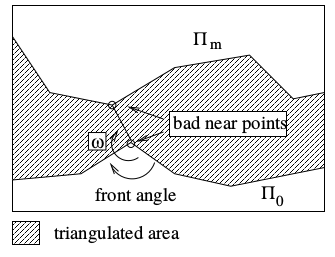
\includegraphics[scale=0.5]{images/hartmann4.png}
\caption{Puntos cercanos \textit{malos} y su detección.}
\end{figure}
\newpage
\begin{enumerate}
\item Determinamos los vecinos $v_1$ y $v_2$ de $p_{0m}$.
\item Determinamos el número $n_t$ de triángulos que van a ser generados:
$$n_t := \mathtt{trunc}\left( \frac{3\omega}{\pi} \right) + 1 \hspace{0.5cm} \text{y} \hspace{0.5cm} \Delta \omega := \frac{\omega}{n_t}$$
Corrección de $\Delta \omega$ para casos extremos:
\begin{itemize}
\item Si $\Delta \omega < 0.8$ y $n_t > 1$ entonces $n_t \to n_t - 1$ y $\Delta \omega = \frac{\omega}{n_t}$.
\item Si $\Delta \omega < 0.8$, $n_t = 1$ y $\| v_1 - v_2 \| > \frac{5}{4} \delta_t$ entonces $n_t = 2$ y $\Delta \omega \to \frac{\Delta \omega}{2}$.
\item Si $\omega < 3$ y $\| v_1 - p_{0m} \| \leq \frac{1}{2} \delta_t$ (ó $\| v_1 - p_{0m} \| \leq \frac{1}{2} \delta_t$) entonces $n_t = 1$.
\end{itemize}

\begin{figure}[h]
\centering
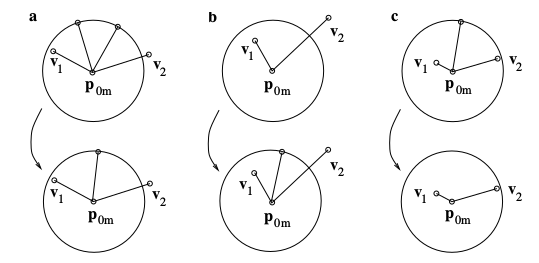
\includegraphics[scale=0.5]{images/hartmann5.png}
\caption{Correcciones de los casos extremos.}
\end{figure}

\item Generamos los triángulos:

Si $n_t = 1$ entonces tenemos un nuevo triángulo $(v_1, v_2, p_{0m})$ en otro caso sean $q_0$ y $q_{n_t}$ las proyecciones ortogonales de $v_1$ y $v_2$ en el plano tangente en el punto $p_{0m}$ y sea $q_i$ el resultado de una rotación de ángulo $i \Delta \omega$ alrededor del normal a la superficie en $p_{0m}$ aplicada a $p_{0m} + \delta_t \frac{q_0 - p_{0m}}{\| q_0 - p_{0m} \|}$. Aplicando el procedimiento \texttt{surfacepoint} a $q_i$ obtendremos nuevo puntos $p_{N+i}$ $i = 1, \dotso, n_t -1$, donde $N$ es el total de puntos existentes hasta el momento, y $n_t$ nuevos triángulos.

\item Renovamos el polígono $\Pi_0$:

Borramos el punto $p_{0m}$ y, si $n_t > 1$, insertamos en su posición los nuevos puntos $p_{N+1}, \dotso, p_{N+n_t-1}$. Todas las variables booleanas tiene el valor \texttt{true} para asegurarnos de que los nuevos cálculos se realizan.
\end{enumerate}
\newpage
\subsubsection{Ejemplos de superficies trianguladas}

\textbf{Esfera}
\[\]
Triangulación de la esfera $x^2 + y^2 + z^2 - 4 = 0$ comenzando por el punto $(1,1,1)$ y paso de longitud $\delta_t = 0.3$. La siguiente imagen muestra los primeros cuatro polígonos delanteros y la situación tras 101 y 1531 triángulos. La triangulación total involucra 1534 triángulos.
\[\]
\begin{figure}[h]
\centering
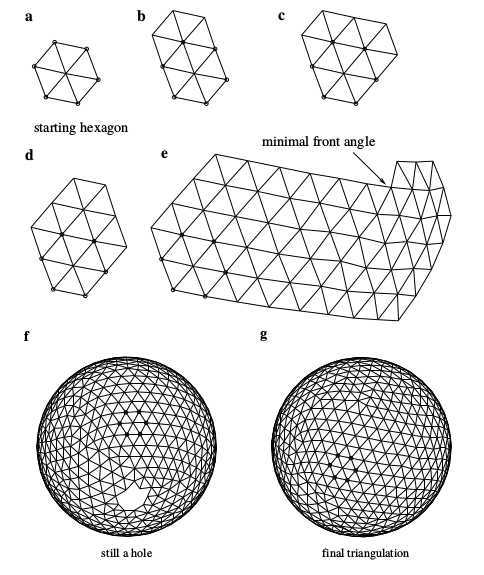
\includegraphics[scale=0.7]{images/hartmann6.png}
\caption{Proceso de triangulación de la esfera.}
\end{figure}

\newpage
\textbf{Cilindro}
\[\]
Triangulación del cilindro $x^2 + y^2 - 1 = 0$ comenzando por el punto $(1,0,0)$ y paso de longitud $\delta_t = 0.2$. 
\[\]
\begin{figure}[h]
\centering
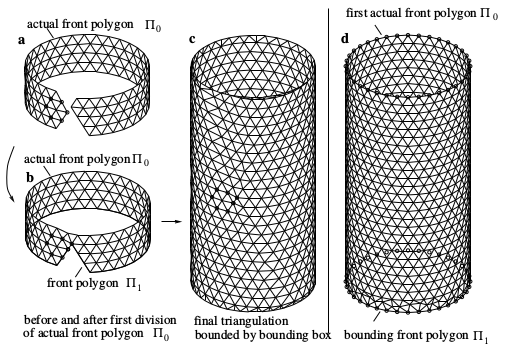
\includegraphics[scale=0.8]{images/hartmann7.png}
\caption{Proceso de triangulación del cilindro.}
\end{figure}

\newpage
\textbf{Toro}
\[\]
Triangulación del cilindro $(x^2+y^2+z^2+0.8775) - 4(x^2+y^2)=0$ comenzando por el punto $(1,0,0.5)$ y paso de longitud $\delta_t = 0.1$.
\[\]

\begin{figure}[h]
\centering
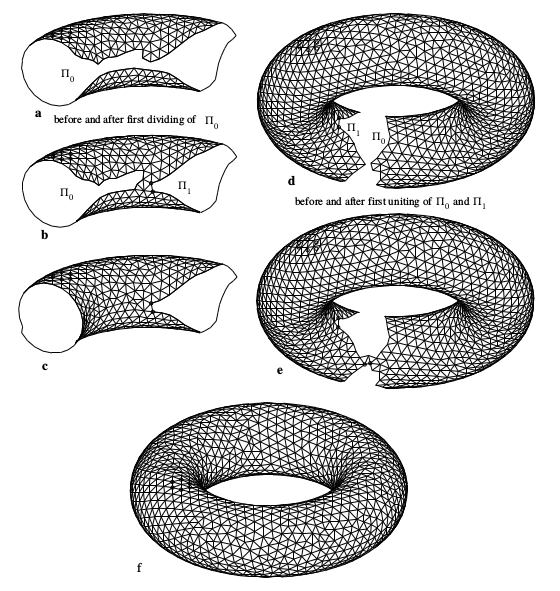
\includegraphics[scale=0.7]{images/hartmann8.png}
\caption{Proceso de triangulación del toro.}
\end{figure}

\newpage
\subsection{Ray Tracing en superficies implícitas}

En 1980, Whitted\cite{Whitted80} propuso un método para generar imágenes de alta calidad usando modelos geométricos básicos. Este método evolucionó en lo que hoy se conoce como Ray Tracing, donde la interacción entre rayos de luz y objetos en la naturaleza es simulado: la luz, ya sea artificial o natural, rebota con los objetos y esto es lo que llega a nuestros ojos e interpretamos las propiedades de los objetos, véase color, transparencia, brillo... Además la luz indirecta puede rebotar en varios objetos antes de llegar a nuestros ojos.

\begin{figure}[h]
\centering
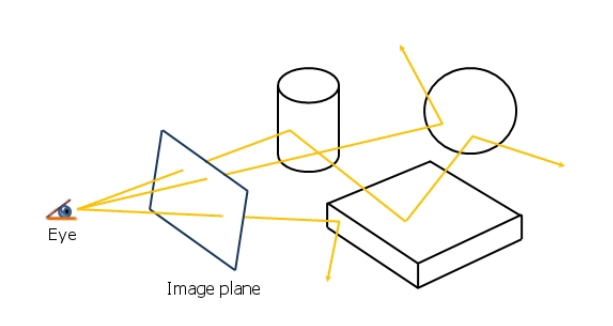
\includegraphics[scale=0.5]{images/florez1.png}
\caption{Rayos de luz rebotando en distintos objetos antes de llegar a nuestros ojos. El plano imagen en la figura se ve cruzado por los rayos; este plano puede contener una representación bidimensional de la escena tridimensional.}
\end{figure}

Usando esta técnica de renderización es posible obtener una representación realista de  de distintos tipos de escenas.
\par En la naturaleza la luz proviene de las llamadas fuentes de luz y, tras rebotar en los objetos del medio, algunos de los rayos llegan a nuestros ojos. Por tanto, analizando el problema, podemos darnos cuenta que, computacionalmente hablando, es muy costoso intentar simular todos los rayos provenientes del foco de luz basándonos en que muchos de los rayos nunca llegarán a nuestro ojo. Por esa razón  es mejor modelar el proceso inverso, esto es, trazar los rayos desde el ojo y buscar las intersecciones con  los objetos del medio.

\subsection{El algoritmo de Ray Tracing}

El método del Ray Tracing es de los llamados{ \em píxel a píxel}. Uno o más rayos de luz son trazados en cada uno de los píxeles en un plano imagen o pantalla. El objetivo es encontrar las intersecciones con los objetos del medio conforme vayamos realizando el trazado de los rayos. Generalmente se suele buscar la primera intersección ya que, en caso de haber más de una, suelen estar obstruidas por el propio objeto.

En la figura \ref{florez27} introducimos el proceso de construcción de un rayo. El punto $c$ representa el origen. Un rayo que comienza en este punto se envía a través de un píxel en la pantalla con dirección $\vec{cs}$. Estos rayos tienen coordenadas con respecto al sistema $uvw$, mientras que el objeto tiene su propio sistema de referencia $xyz$. Esta independencia de los sistemas de referencia permite ver la escena desde cualquier posición arbitraria.

\begin{figure}[h]
\centering
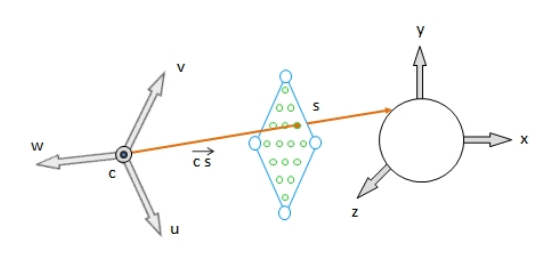
\includegraphics[scale=0.5]{images/florez2.png}
\caption{Definición de un rayo cruzando una pantalla. Si el rayo interseca alguna superficie, el color se calcula y asignado al píxel en la pantalla.}
\label{florez27}
\end{figure}

Si hay alguna intersección entre el rayo y el objeto el color es calculando tomando en cuenta la dirección del vector normal del punto de intersección y la posición de las luces. La aportación de las luces indirectas también se calcula. La suma de todas las posibles aportaciones se usa para asignar el color correspondiente en el píxel.

\textbf{Análisis de la intersección}

Un rayo se define como
\begin{equation}
\begin{split}
x = c_x + t(x_s - c_x), \\
y = c_y + t(y_s - c_y), \\
z = c_z + t(y_z - c_z).
\end{split}
\nonumber
\end{equation}
Donde $(c_x,c_y,c_z)$ es origen o punto de vista, $(x_s,y_s,z_s)$ es el punto donde el rayo cruza la pantalla y $t$ es el parámetro del rayo.

La intersección entre la superficie implícita $f(x,y,z) = 0$ y el rayo viene definida por la ecuación
$$g(t) = 0,$$
donde $g(t)$ es la función $g : \mathbb{R}_0 \to \mathbb{R}^3$ definida por
\begin{equation}
g(t) \equiv f(c_x + t(x_s - c_x), c_y + t(y_s - c_y), c_z + t(y_z - c_z)).
\nonumber
\end{equation}
De este modo, el problema se reduce a encontrar las raíces de la función $g$.

Estas soluciones se sustituyen en la definición paramétrica del rayo para encontrar el punto de intersección y el valor del vector normal.

Existen muchas maneras  de encontrar las raíces de $g$. Las manera más clásicas son el método de la bisección o de Newton\cite{Hart01}. También existen de otro tipo como: técnicas fuzzy\cite{Foufou96}, aritmética de intervalos\cite{Mitchell90} o constantes de Lipschitz\cite{Kalra89}.
\subsection{Ray Tracing eficiente}

Como ya hemos comentado el principal problema del algoritmo de Ray Tracing es la falta de eficiencia. Muchos autores han propuesto diferentes técnicas de mejora de la eficiencia pero se pueden clasificar en tres grupos:
\begin{itemize}
\item Intersecciones más rápidas.
\item Trazar menor cantidad de rayos.
\item Generalización de los rayos.
\end{itemize}

La técnica más básica para acelerar el Ray Tracing es el llamado{ \em volumen delimitador o límite},que consiste en crear un volumen que contenga a nuestro objeto y que el cálculo de la intersección de los rayos con éste sea menos costoso que con el objeto en sí. La primera propuesta de volumen delimitador fue la esfera\cite{Whitted80} por la simplicidad y por la facilidad para probar la intersección de los rayos con ésta. La idea es recubrir cada objeto con una esfera, si un rayo interseca a una esfera, entonces se analiza el caso dentro de la esfera, en caso contrario no es necesario. Si además añadimos lo que se suele llamar{ \em jerarquía} el orden del algoritmo se puede reducir a $log(n)$.

Otra técnica bastante común en la literatura especializada es la subdivisión del espacio en la cual el espacio que rodea a nuestro objeto se divide y se descartan las subdivisiones que no contienen parte del objeto alguno. Podemos dividir el espacio de manera regular o de manera adaptativa como con la poligonalización, pero conlleva los mismos inconvenientes.\\ La ventaja que  tiene este método es que, al ordenar las divisiones, sólo hay que probar el rayo para cada una de éstas en lugar de para el espacio completo para buscar la primera intersección.

Ya como final tenemos las llamadas técnicas direccionales en la que se mejora la técnica anterior discretizando también las direcciones.

\section{Conclusiones}

En este capítulo hemos visto distintas maneras de representar y visualizar superficies expresadas de forma implícita, de las cuales ya hemos nombrado sus ventajas e inconvenientes. En términos de coste computacional y velocidad de renderización éstas no presentan ningún reto y presentan una serie de propiedades que las hacen muy atractivas.

En el siguiente capítulo haremos una introducción al Análisis de Intervalos para mejorar la capacidad de computación y tratar de solventar los problemas de redondeo de las máquinas debido a los puntos flotantes.